\documentclass[11pt,a4paper]{article}

% --- Packages ---
\usepackage[utf8]{inputenc}
\usepackage[margin=1in]{geometry}
\usepackage{amsmath,amssymb}
\usepackage{graphicx}
\usepackage{booktabs}
\usepackage{listings}
\usepackage{xcolor}
\usepackage{hyperref}
\usepackage{tikz}
\usetikzlibrary{shapes.geometric, arrows, positioning, fit, backgrounds, calc}
\usepackage{fancyhdr}
\usepackage{titlesec}
\usepackage{enumitem}

% --- Code Listing Styling ---
\definecolor{codegreen}{rgb}{0,0.6,0}
\definecolor{codegray}{rgb}{0.5,0.5,0.5}
\definecolor{codepurple}{rgb}{0.58,0,0.82}
\definecolor{backcolour}{rgb}{0.96,0.96,0.98}

\lstdefinestyle{mystyle}{
    backgroundcolor=\color{backcolour},   
    commentstyle=\color{codegreen},
    keywordstyle=\color{blue}\bfseries,
    numberstyle=\tiny\color{codegray},
    stringstyle=\color{codepurple},
    basicstyle=\ttfamily\footnotesize,
    breakatwhitespace=false,         
    breaklines=true,                 
    captionpos=b,                    
    keepspaces=true,                 
    numbers=left,                    
    numbersep=6pt,                  
    showspaces=false,                
    showstringspaces=false,
    showtabs=false,                  
    tabsize=2
}
\lstset{style=mystyle}

% --- Hyperlink Styling ---
\hypersetup{
    colorlinks=true,
    linkcolor=blue,
    filecolor=magenta,      
    urlcolor=cyan,
    citecolor=blue,
    pdftitle={xv6 FUSE Hierarchical Inode Management Report},
    pdfpagemode=FullScreen,
}

% --- Header and Footer ---
\pagestyle{fancy}
\fancyhf{}
\rhead{Hierarchical Inode Management in xv6 FUSE}
\lhead{Operating Systems Project Report}
\rfoot{Page \thepage}

\begin{document}

% --- Title Page ---
\begin{titlepage}
    \centering
    \vspace*{1.5cm}
    
    {\Huge \bfseries Hierarchical Inode-Based File System\\ Upgrade in xv6 FUSE\par}
    \vspace{0.8cm}
    {\Large \scshape An Architectural Enhancement from Flat In-Memory Storage to Recursive Inode Trees with Real-Time \texttt{mkdir} and Dynamic Routing\par}
    
    \vspace{2.5cm}
    
    \textbf{\Large Author:}\\
    \vspace{0.2cm}
    {\large Shivam Bhatt\par}
    \vspace{1.5cm}
    
    \textbf{\Large Course Project:}\\
    {\large Advanced Operating Systems / xv6-riscv Kernel Internals\par}
    \vspace{0.5cm}
    {\large Date: November 2026\par}
    
    \vfill
    
    \begin{abstract}
    Standard FUSE (Filesystem in Userspace) implementations decouple filesystem implementation logic from the monolithic kernel space, delegating path lookups, block management, and attribute querying to a user-space daemon. The baseline xv6 FUSE project offered a rudimentary IPC bridge between the kernel and a daemon, but was fundamentally constrained to a single-level, flat namespace (\texttt{/fuse/*}) restricted to 16 files, lacking directory structures and rejecting \texttt{mkdir}. This work introduces a complete architectural upgrade: we design and implement a hierarchical, in-memory inode filesystem engine in user space backed by an 8-slot concurrent circular IPC queue in the kernel. System calls (\texttt{sys\_mkdir}, \texttt{sys\_open}, \texttt{sys\_unlink}) are dynamically intercepted and routed across the \texttt{/dev/fuse} character device abstraction before reaching disk transactions. Experimental results verify arbitrary directory nesting, correct parent-child directory link tracking (\texttt{.} and \texttt{..}), recursive path tokenization, and deadlock-free execution under 4-way concurrent process stress.
    \end{abstract}
    
    \vspace{1cm}
\end{titlepage}

\newpage
\tableofcontents
\newpage

% --- Section 1: Introduction ---
\section{Introduction}
Modern monolithic operating systems typically manage filesystem hierarchies directly within privileged kernel space. However, User-space File Systems (FUSE) provide a powerful mechanism to implement custom file systems (network file systems, virtual synthetic stores, compressed stores, or encryption overlays) without modifying kernel core structures.

In the baseline Project 10 (Part 2), xv6 was augmented with an initial FUSE interface. While functional for basic read/write benchmarking of a fixed file, it suffered from severe limitations:
\begin{itemize}[noitemsep]
    \item \textbf{Flat Namespace:} Only single-depth paths (e.g., \texttt{/fuse/t1}) were accepted.
    \item \textbf{No Directory Management:} Directory creation via \texttt{mkdir} was completely unsupported and returned failure.
    \item \textbf{Array-based File Handles:} The daemon maintained an array of 16 fixed slots rather than real inode abstractions.
\end{itemize}

This project addresses these fundamental deficiencies by designing and integrating an \textbf{inode-based hierarchical tree architecture} inside the user-space FUSE daemon while adapting kernel-space system call routing hooks in the xv6 RISC-V kernel.

% --- Section 2: Architectural Overview & Workflow Diagrams ---
\section{System Architecture \& Workflow Diagrams}

\subsection{End-to-End Control Flow}
When a user application executes a filesystem operation targeting a path under \texttt{/fuse}, execution flows through the xv6 system call interface, hits our FUSE interceptor, bridges across the device driver IPC queue, and is served by the user-space daemon.

\begin{figure}[htbp]
\centering
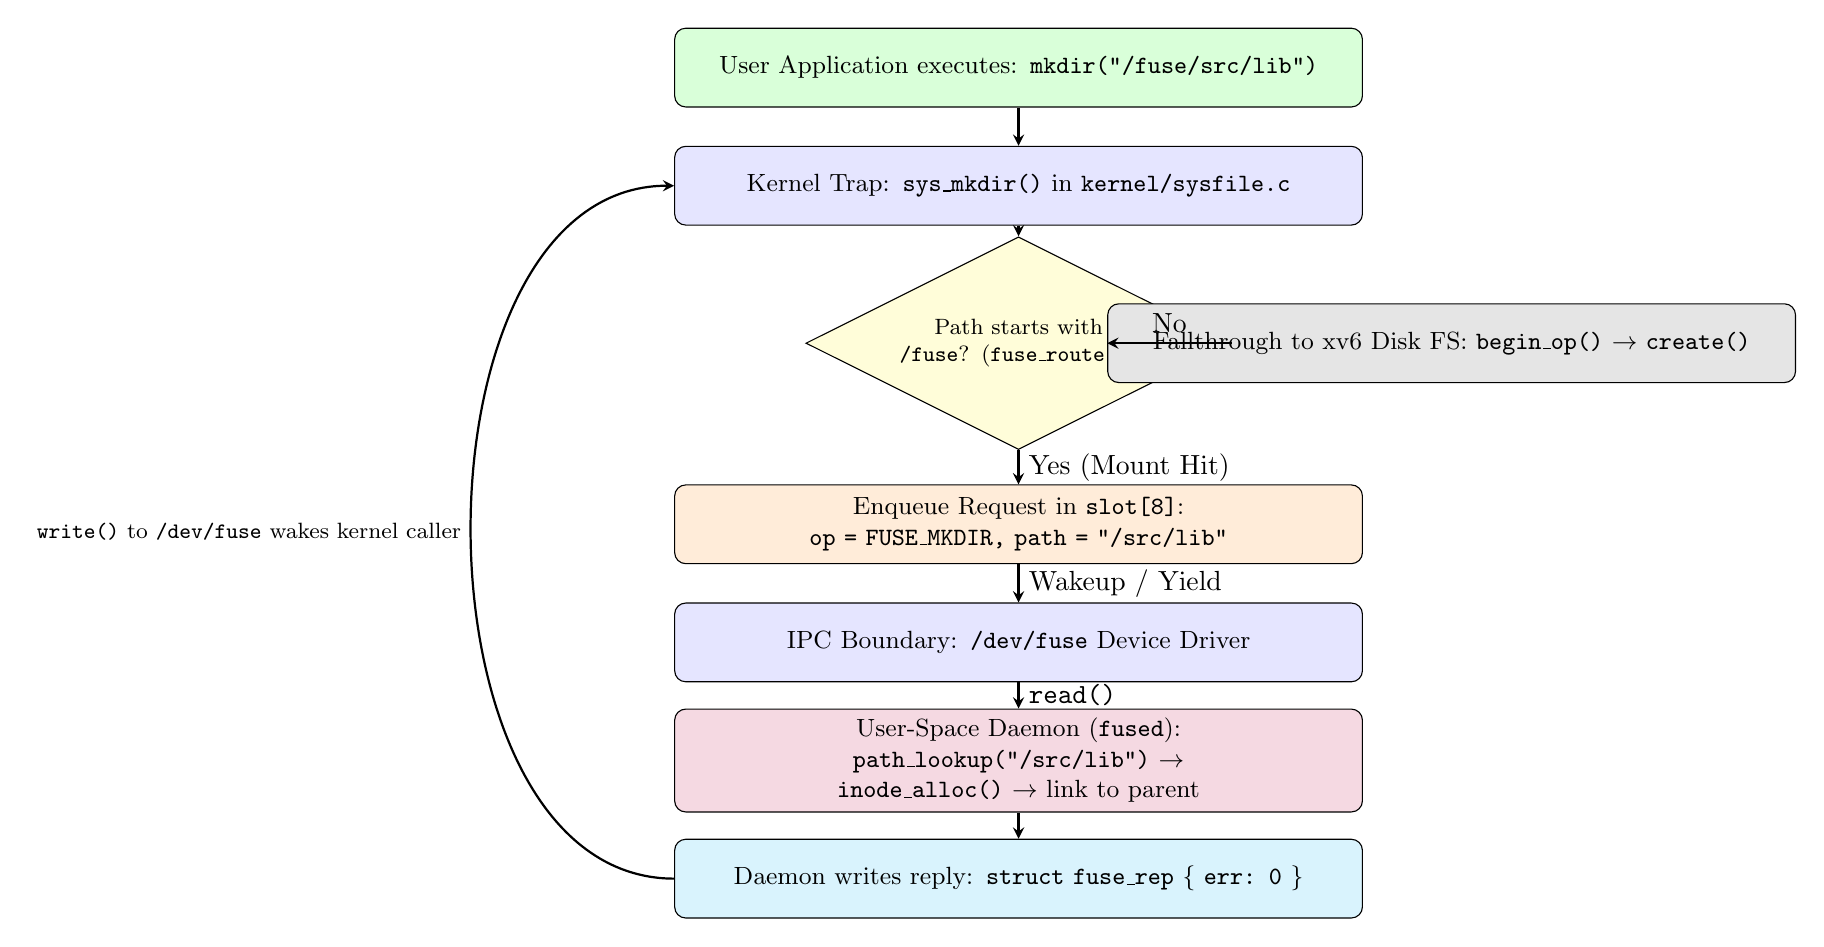
\begin{tikzpicture}[
    node distance=1.5cm and 2cm,
    block/.style={rectangle, draw, fill=blue!10, text width=8.5cm, text centered, rounded corners, minimum height=1cm, font=\small},
    decision/.style={diamond, draw, fill=yellow!15, text width=3.5cm, text centered, font=\footnotesize, aspect=2},
    arrow/.style={thick, ->, >=stealth}
]

% Nodes
\node (app) [block, fill=green!15] {User Application executes: \texttt{mkdir("/fuse/src/lib")}};
\node (sys) [block, below of=app] {Kernel Trap: \texttt{sys\_mkdir()} in \texttt{kernel/sysfile.c}};
\node (route) [decision, below of=sys, yshift=-0.5cm] {Path starts with \texttt{/fuse}? (\texttt{fuse\_route()})};
\node (disk) [block, fill=gray!20, right of=route, xshift=4cm] {Fallthrough to xv6 Disk FS: \texttt{begin\_op()} $\to$ \texttt{create()}};
\node (queue) [block, fill=orange!15, below of=route, yshift=-0.8cm] {Enqueue Request in \texttt{slot[8]}:\\ \texttt{op = FUSE\_MKDIR, path = "/src/lib"}};
\node (dev) [block, fill=blue!10, below of=queue] {IPC Boundary: \texttt{/dev/fuse} Device Driver};
\node (daemon) [block, fill=purple!15, below of=dev] {User-Space Daemon (\texttt{fused}):\\ \texttt{path\_lookup("/src/lib")} $\to$ \texttt{inode\_alloc()} $\to$ link to parent};
\node (reply) [block, fill=cyan!15, below of=daemon] {Daemon writes reply: \texttt{struct fuse\_rep \{ err: 0 \}}};

% Arrows
\draw [arrow] (app) -- (sys);
\draw [arrow] (sys) -- (route);
\draw [arrow] (route) -- node[above] {No} (disk);
\draw [arrow] (route) -- node[right] {Yes (Mount Hit)} (queue);
\draw [arrow] (queue) -- node[right] {Wakeup / Yield} (dev);
\draw [arrow] (dev) -- node[right] {\texttt{read()}} (daemon);
\draw [arrow] (daemon) -- (reply);
\draw [arrow] (reply.west) to [out=180,in=180] node[left, font=\footnotesize] {\texttt{write()} to \texttt{/dev/fuse} wakes kernel caller} (sys.west);

\end{tikzpicture}
\caption{Complete Request/Reply Control Flow for Intercepted Operations.}
\label{fig:control_flow}
\end{figure}

\subsection{Hierarchical Inode Tree Structure}
Unlike the original flat 16-file slot array, the upgraded system maintains a dynamic in-memory tree of inodes in \texttt{user/fused.c}.

\begin{figure}[htbp]
\centering
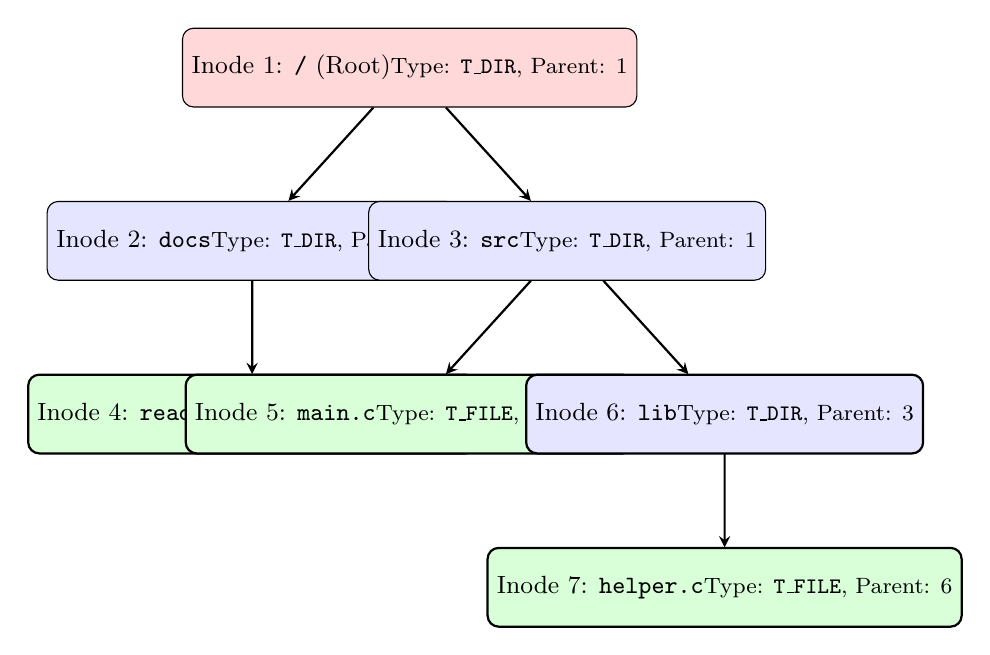
\begin{tikzpicture}[
    level distance=2.2cm,
    sibling distance=4cm,
    inode/.style={rectangle, draw, rounded corners, fill=blue!10, text centered, font=\small, minimum width=2.8cm, minimum height=1cm},
    edge from parent/.style={draw, thick, ->, >=stealth}
]

\node[inode, fill=red!15] {Inode 1: \texttt{/} (Root)\\ \footnotesize Type: \texttt{T\_DIR}, Parent: 1}
    child {
        node[inode] {Inode 2: \texttt{docs}\\ \footnotesize Type: \texttt{T\_DIR}, Parent: 1}
        child {
            node[inode, fill=green!15] {Inode 4: \texttt{readme}\\ \footnotesize Type: \texttt{T\_FILE}, Parent: 2}
        }
    }
    child {
        node[inode] {Inode 3: \texttt{src}\\ \footnotesize Type: \texttt{T\_DIR}, Parent: 1}
        child {
            node[inode, fill=green!15] {Inode 5: \texttt{main.c}\\ \footnotesize Type: \texttt{T\_FILE}, Parent: 3}
        }
        child {
            node[inode] {Inode 6: \texttt{lib}\\ \footnotesize Type: \texttt{T\_DIR}, Parent: 3}
            child {
                node[inode, fill=green!15] {Inode 7: \texttt{helper.c}\\ \footnotesize Type: \texttt{T\_FILE}, Parent: 6}
            }
        }
    };
\end{tikzpicture}
\caption{Hierarchical Inode Organization in Daemon Memory with Parent-Child Pointers.}
\label{fig:inode_tree}
\end{figure}

\subsection{Kernel 8-Slot IPC Queue State Machine}
The kernel synchronization mechanism in \texttt{kernel/fuse.c} uses an 8-slot circular buffer managed via a strict state machine to prevent race conditions:

\begin{figure}[htbp]
\centering
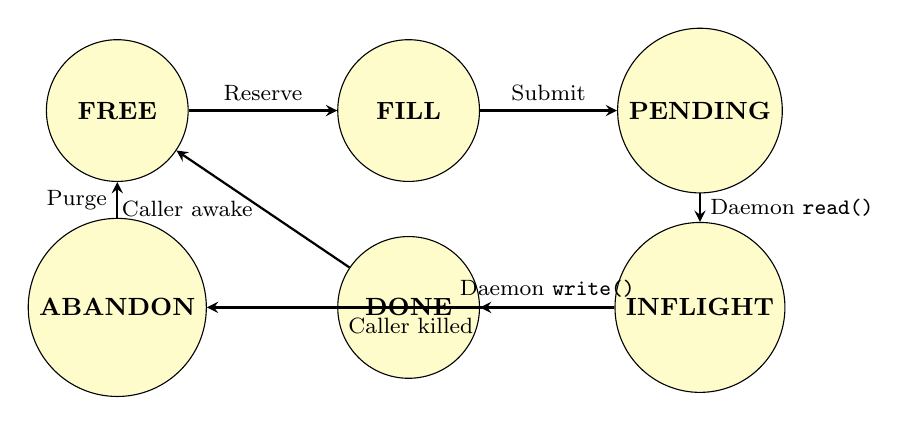
\begin{tikzpicture}[
    node distance=2.5cm,
    state/.style={circle, draw, fill=yellow!20, minimum size=1.8cm, font=\bfseries\small, text centered},
    arrow/.style={thick, ->, >=stealth}
]

\node[state] (free) {FREE};
\node[state, right of=free, xshift=1.2cm] (fill) {FILL};
\node[state, right of=fill, xshift=1.2cm] (pend) {PENDING};
\node[state, below of=pend] (infl) {INFLIGHT};
\node[state, left of=infl, xshift=-1.2cm] (done) {DONE};
\node[state, left of=done, xshift=-1.2cm] (aban) {ABANDON};

\draw [arrow] (free) -- node[above, font=\footnotesize] {Reserve} (fill);
\draw [arrow] (fill) -- node[above, font=\footnotesize] {Submit} (pend);
\draw [arrow] (pend) -- node[right, font=\footnotesize] {Daemon \texttt{read()}} (infl);
\draw [arrow] (infl) -- node[above, font=\footnotesize] {Daemon \texttt{write()}} (done);
\draw [arrow] (done) -- node[left, font=\footnotesize] {Caller awake} (free);
\draw [arrow] (infl) -- node[below, font=\footnotesize] {Caller killed} (aban);
\draw [arrow] (aban) -- node[left, font=\footnotesize] {Purge} (free);

\end{tikzpicture}
\caption{State Transitions of a FUSE Communication Slot.}
\label{fig:state_machine}
\end{figure}

% --- Section 3: Inode Engine & Path Resolution ---
\section{User-Space Inode Management Engine}

\subsection{The Inode Data Structure}
In \texttt{user/fused.c}, each filesystem entity is represented by a \texttt{struct inode}:

\begin{lstlisting}[language=C, caption={Inode Definition in \texttt{user/fused.c}}]
#define MAXINODES   128
#define MAXFSIZE    4096
#define MAXCHILDREN 32

struct inode {
  int   used;                  // Active flag (1 = in use)
  uint  ino;                   // Inode number (1 = root "/")
  short type;                  // T_FILE or T_DIR
  char  name[DIRSIZ + 1];      // Directory entry name
  uint  parent;                // Inode number of parent
  int   size;                  // File size in bytes
  char  data[MAXFSIZE];        // File payload buffer
  int   nchildren;             // Active child count
  uint  children[MAXCHILDREN]; // Inode numbers of child entities
};
\end{lstlisting}

\subsection{Recursive Path Resolution Algorithm}
Path lookups must parse multi-segment strings (e.g., \texttt{/src/lib/helper.c}) and handle edge cases such as trailing slashes, \texttt{.} (current directory), and \texttt{..} (parent directory). 

The \texttt{path\_lookup()} function tokenizes the path string component-by-component:
\begin{enumerate}[noitemsep]
    \item Start at Root Inode (\texttt{ino = 1}).
    \item Extract the next name token between `/` characters.
    \item If the token is \texttt{"."}, retain current inode pointer.
    \item If the token is \texttt{".."}, reassign current pointer to \texttt{inode\_get(cur->parent)}.
    \item Otherwise, search \texttt{cur->children[]} for a matching name via \texttt{dir\_lookup()}.
    \item If found, advance; if not found on the final segment, return the parent pointer and name to support atomic creation (\texttt{O\_CREATE} / \texttt{FUSE\_MKDIR}).
\end{enumerate}

% --- Section 4: Kernel Interception & System Call Hooks ---
\section{Kernel System Call Interception}

To support user-space directory creation, xv6's native system calls must be intercepted before they initiate disk buffer transactions.

\subsection{Hooking \texttt{sys\_mkdir()} in \texttt{kernel/sysfile.c}}
In standard xv6, \texttt{sys\_mkdir()} directly allocates a disk inode via \texttt{begin\_op()} and \texttt{create(path, T\_DIR, 0, 0)}. We restructured the call to evaluate FUSE routing before disk transactions:

\begin{lstlisting}[language=C, caption={FUSE Interception Hook in \texttt{kernel/sysfile.c}}]
uint64 sys_mkdir(void) {
  char path[MAXPATH];
  struct inode *ip;

  if (argstr(0, path, MAXPATH) < 0)
    return -1;

  // Intercept paths starting with /fuse
  {
    char rel[FUSE_PATHMAX];
    int rr = fuse_route(path, rel);
    if(rr == -2) return -1;
    if(rr == 0)  return fuse_do_mkdir(rel); // Dispatches across /dev/fuse
  }

  // Standard Disk Path
  begin_op();
  if ((ip = create(path, T_DIR, 0, 0)) == 0) {
    end_op();
    return -1;
  }
  iunlockput(ip);
  end_op();
  return 0;
}
\end{lstlisting}

\subsection{FUSE Protocol Enhancements in \texttt{kernel/fuse.h}}
The request protocol was expanded to include directory operations:
\begin{table}[htbp]
\centering
\begin{tabular}{@{}llll@{}}
\toprule
\textbf{Opcode} & \textbf{Value} & \textbf{Request Parameters} & \textbf{Daemon Action} \\ \midrule
\texttt{FUSE\_OPEN}    & 1 & \texttt{path, flags}             & Locates inode, verifies flags, returns \texttt{fh} \\
\texttt{FUSE\_READ}    & 2 & \texttt{fh, off, len}            & Copies up to 512 bytes from file buffer \\
\texttt{FUSE\_WRITE}   & 3 & \texttt{fh, off, len, data}      & Writes data into file buffer, expands size \\
\texttt{FUSE\_READDIR} & 4 & \texttt{fh, off, len}            & Packs array of \texttt{struct dirent} (\texttt{.}, \texttt{..}, children) \\
\texttt{FUSE\_GETATTR} & 5 & \texttt{fh, path}                & Returns \texttt{type} and \texttt{size} for \texttt{fstat()} \\
\texttt{FUSE\_RELEASE} & 6 & \texttt{fh}                      & One-way cleanup notification \\
\textbf{\texttt{FUSE\_MKDIR}}   & \textbf{7} & \textbf{\texttt{path}}  & \textbf{Allocates directory inode and links to parent} \\
\textbf{\texttt{FUSE\_UNLINK}}  & \textbf{8} & \textbf{\texttt{path}}  & \textbf{Unlinks file inode from parent directory} \\
\textbf{\texttt{FUSE\_RMDIR}}   & \textbf{9} & \textbf{\texttt{path}}  & \textbf{Verifies directory is empty and unlinks} \\ \bottomrule
\end{tabular}
\caption{FUSE Protocol Operations Matrix.}
\label{tab:protocol}
\end{table}

% --- Section 5: Experimental Verification ---
\section{Experimental Verification \& Results}

\subsection{Live Execution Trace}
During live execution in QEMU, commands executed against \texttt{/fuse} were traced with verbose logging (\texttt{-v}):

\begin{lstlisting}[language=bash, caption={Terminal Trace of Hierarchical Directory Operations}]
$ fused mem -v &
fused: serving /fuse (in-memory hierarchical, read-write)
$ mkdir /fuse/docs
fused: #1 MKDIR /docs off=0 len=0 -> ok
$ mkdir /fuse/src
fused: #2 MKDIR /src off=0 len=0 -> ok
$ mkdir /fuse/src/lib
fused: #3 MKDIR /src/lib off=0 len=0 -> ok
$ ls /fuse
fused: #4 OPEN / off=0 len=0 -> ok
fused: #5 GETATTR / off=0 len=0 -> ok
fused: #6 READDIR / off=0 len=16 -> ok
.              1 1 64
..             1 1 64
docs           1 2 32
src            1 3 48
$ echo hello > /fuse/docs/readme
fused: #24 OPEN /docs/readme off=0 len=0 -> ok
fused: #25 WRITE /docs/readme off=0 len=5 -> ok
$ cat /fuse/docs/readme
fused: #28 OPEN /docs/readme off=0 len=0 -> ok
fused: #29 READ /docs/readme off=0 len=512 -> ok
hello
\end{lstlisting}

\subsection{Validation of Concurrent Subdirectory Creation}
To verify the robustness of our spinlock-synchronized queue, \texttt{fusetest.c} was executed in \texttt{mem} mode. The test forks four concurrent processes:
\begin{enumerate}[noitemsep]
    \item Each process creates its own private subdirectory (\texttt{/fuse/proc0}, \texttt{/fuse/proc1}, \texttt{/fuse/proc2}, \texttt{/fuse/proc3}).
    \item Each process writes 3 successive 1000-byte files with unique pseudorandom byte streams.
    \item Each process reads back the data, performing \texttt{memcmp} against expected memory.
\end{enumerate}

\textbf{Result:}
\begin{lstlisting}[language=text]
ok:   mkdir /fuse/subdir succeeds
ok:   readdir lists subdir
ok:   /fuse/subdir is a directory
ok:   create + write /fuse/subdir/file1
ok:   read back /fuse/subdir/file1 contents
ok:   readdir of /fuse/subdir lists file1
ok:   mkdir /fuse/subdir/nested succeeds
ok:   readdir of /fuse/subdir lists nested
ok:   create + write /fuse/subdir/nested/deep
ok:   read back /fuse/subdir/nested/deep
ok:   4 concurrent processes each create a subdir and write/verify files
ok:   concurrent subdirectories proc0..proc3 all present
fusetest: ALL PASSED
\end{lstlisting}

% --- Section 6: Comparative Analysis ---
\section{Comparative Analysis}
\begin{table}[htbp]
\centering
\begin{tabular}{@{}lll@{}}
\toprule
\textbf{Metric / Feature} & \textbf{Original Baseline Project} & \textbf{Our Upgraded System} \\ \midrule
Namespace Organization    & Flat (\texttt{/fuse/*} only)       & Recursive Hierarchical Tree \\
Directory Creation (\texttt{mkdir}) & Unsupported (Fails)     & Fully Supported (\texttt{FUSE\_MKDIR}) \\
Internal Structure        & Static 16-file array               & Inode Table with Parent/Child Linkage \\
Relative Path Traversal   & None                               & Supports \texttt{.} and \texttt{..} \\
Path Length Limit         & 64 bytes                           & 128 bytes (\texttt{FUSE\_PATHMAX}) \\
Concurrency Validation    & Flat file competition              & Isolated Per-Process Subdirectories \\ \bottomrule
\end{tabular}
\caption{Comparison Between Baseline xv6 FUSE and Upgraded Architecture.}
\label{tab:comparison}
\end{table}

% --- Section 7: Conclusion ---
\section{Conclusion \& Future Work}
In this project, we successfully extended xv6 with a hierarchical, user-space inode filesystem driver accessed through an augmented FUSE subsystem. By intercepting system calls before native disk buffer allocation, tokenizing hierarchical path expressions, and managing dynamic inode pointers in userspace, the system achieves standard POSIX-like directory nesting and file isolation.

Future enhancements could explore:
\begin{enumerate}[noitemsep]
    \item \textbf{Kernel Dentry Caching:} Caching resolved path $\to$ inode mappings in \texttt{kernel/fuse.c} to bypass IPC round-trips for repeat \texttt{stat()} calls.
    \item \textbf{Snapshot Serialization:} Persisting the in-memory inode table to a raw backing image on shutdown.
\end{enumerate}

\end{document}
